\section{Numerical Evaluation and Analysis}
\label{sec:moaexperimentdesign}

To evaluate the performance of heterogeneous wireless network deployment, we perform  
numerical evaluation with linear program, and MHAPD algorithm to analyze the role
of white space and WiFi bands in total access points required for a given deployment 
area.

\subsection{Experimental Setup}

% 4 bands, capacity, individual traffic demand,  
In the evaluation, we set the demand request as 2 Mbps per person with the population
density from 20 to 2000 per square kilometer. We assume $30\%$ residents will use this
service, the maximum transmit power is 30 dBm, and a path loss exponent of $3.5$ from 
Ref.~\cite{meikle2012global}. 

% Channel availability and influence, and in hexagon model
We adopt an 802.11n maximum data rate of 600 Mbps. In the protocol model, the interference 
range is as twice as the communication range. We investigate both traffic demand and the 
number of white space channel influence on heterogeneous wireless network deployment. 
We have interference free scenario, each band has at least 3 channels, which fits for
most rural areas and some cities, such as Houston~\cite{googledatabase}. In this scenario,
it is possible to use all heterogeneous access points since heterogeneous access point could 
serve more area. However, in the field, there are some cities has area only one or two 
licensed white space channel, such as Salt Lake City~\cite{googledatabase}. In these scenario, 
only part of the access points could be heterogeneous. We run numerical simulation of
both the scenarios and analyze the heterogeneous access points amount of the results.

We given the target area as $15\times 15$ square kilometers. In the numerical simulation, 
we assign orthogonal WiFi channels in 2.4 GHz,5.8 GHz and white space 
channels in 450 MHz, 800MHz. Then we calculate the service area of access point according to 
their radio combinations as described in~\ref{subsec:problem} with a hexagonal model. Then we 
run our linear program and MHAPD methods to investigate the benefit from white space band 
and in what degree heterogeneous access point is beater than single radio access point. 


\subsection{Results and Analysis} 
\label{subsec:result}

% Results
Fig.~\ref{fig:enoughchannels} shows access point number to serve the target area when 
the area has more than 3 white space channels, which means white space radios could be used
on all access points in hexagonal deployment model. In the simulation, we set 3 white space channels
in 450 MHz. In this scenario, at the beginning, the served area of WiFi only access point 
is restricted by the communication range. As the population distribution increase, 
the served area of WiFi only access point will be limited by the traffic demand instead 
of the communication range. The curve keeps flat until the traffic demand becomes the limitation
of the served area. In the heterogeneous deployment, the served area is restricted by the traffic
demand at the beginning, the number of access point increase as the traffic demand increase. 
Also since there are enough channels can be reused, our algorithm use almost the same number of 
access point to serve the target area. In this scenario, as population distribution increase,
the gain of adding white space channels in our algorithm comparing with WiFi only(2.4 GHz) 
decrease from 686\% to 248\% and keep around the value 260\%. The gain is from the large 
propagation range of white space bands at low population distribution.
As the population distribution increase, which means the traffic demand increase, some of the gain
comes from more capacity of heterogeneous access point.


\begin{figure}
%\vspace{-0.0in}
\centering
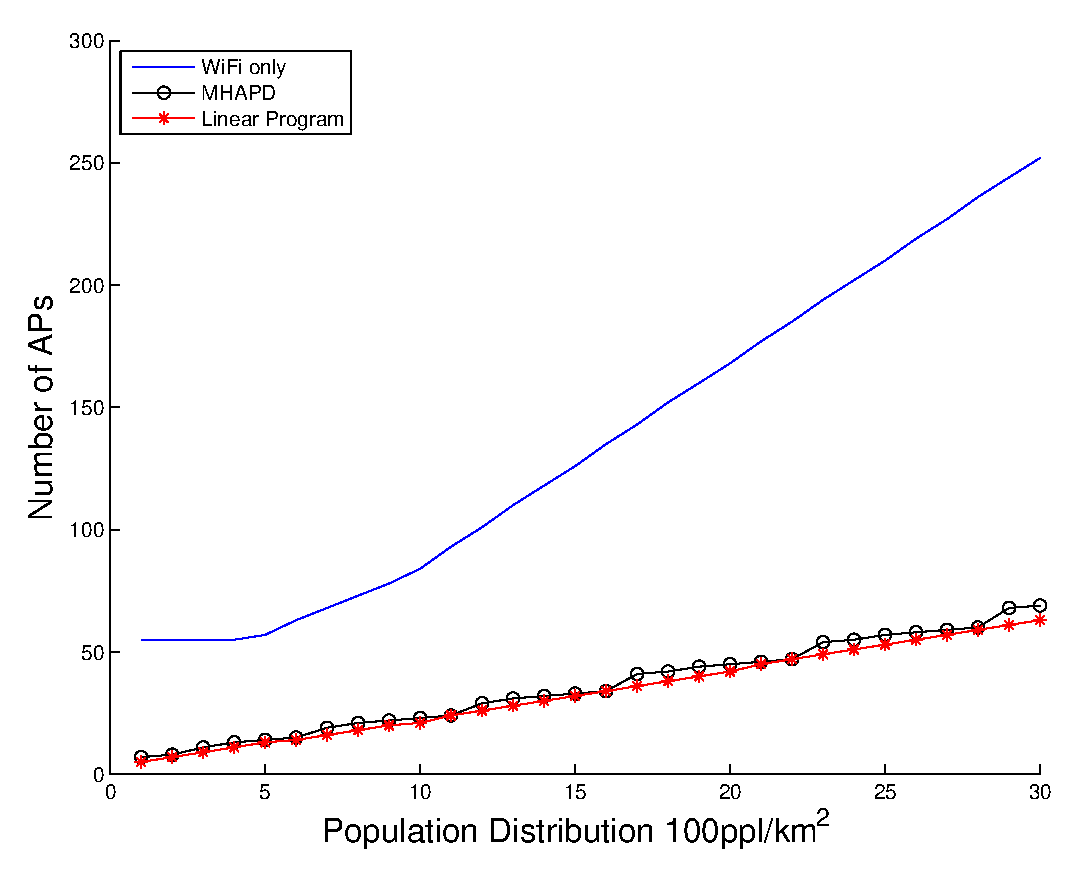
\includegraphics[width=74mm]{figures/enoughchannels}
\vspace{-0.1in}
\caption{Sufficient White Space Channels Scenario}                                                                 
\label{fig:enoughchannels}
\vspace{-0.1in}
\end{figure}

With few white space band Chane's(less than 3 channels), in the hexagonal model, only one or 
two neighbor access point could use white space channel. Fig.~\ref{fig:onewhitechannel}
shows the simulation result of one 450 MHz channel deployment. Shortage of white space channels
make the number of access points much more than the linear program calculation. The gain from 
white space channel is from 323\% to 86\%. 

In these sufficient and shortage of white space channel scenarios, the highest gains are from 
low population distribution. This result represent that white space band fits rural or suburban
area where has few residents. When the population distribution increase, the benefit of white space
channels is from their bandwidth, which is the same as adding more WiFi channels.



\begin{figure}
%\vspace{-0.0in}
\centering
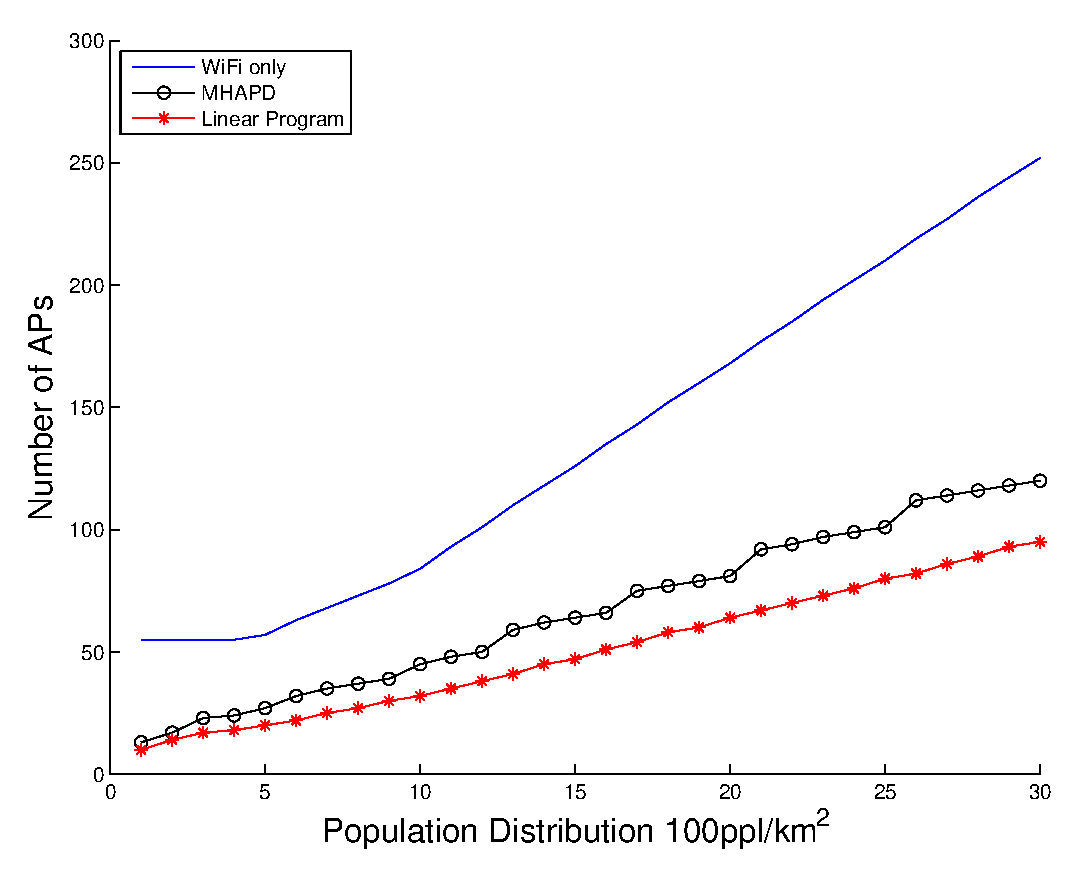
\includegraphics[width=74mm]{figures/onewhitechannel}
\vspace{-0.1in}
\caption{One white channel}                                                                 
\label{fig:onewhitechannel}
\vspace{-0.1in}
\end{figure}

In Fig.~\ref{fig:heappercentage}, we investigate the percentage of heterogeneous access points
in 3 white space channels scenario and two white space channels scenario in our algorithm. 
With sufficient white space channels, we prefer heterogeneous access point and there is no 
limitation of the heterogeneous access point deployment. The percentage of heterogeneous access points
is higher than 80\%. In two white space channels scenario, at the beginning the number of hetergeneous
access point is restricted by the interference range. As the population increase, no more heterogeneous
access point could be added in the target area, we have to add more WiFi access point which makes the 
heterogeneous points percentage decrease. When the population distribution reach the threshold which
the traffic demand restrict the service area of heterogeneous access point, the percentage increases.
When the service area shrink as the WiFi access point, since they have more capacity, all the access
points become heterogeneous. In the white space channel shortage scenario, white space channel becomes
the inside service area of heterogeneous access point to explore spatial reuse.



\begin{figure}
%\vspace{-0.0in}
\centering
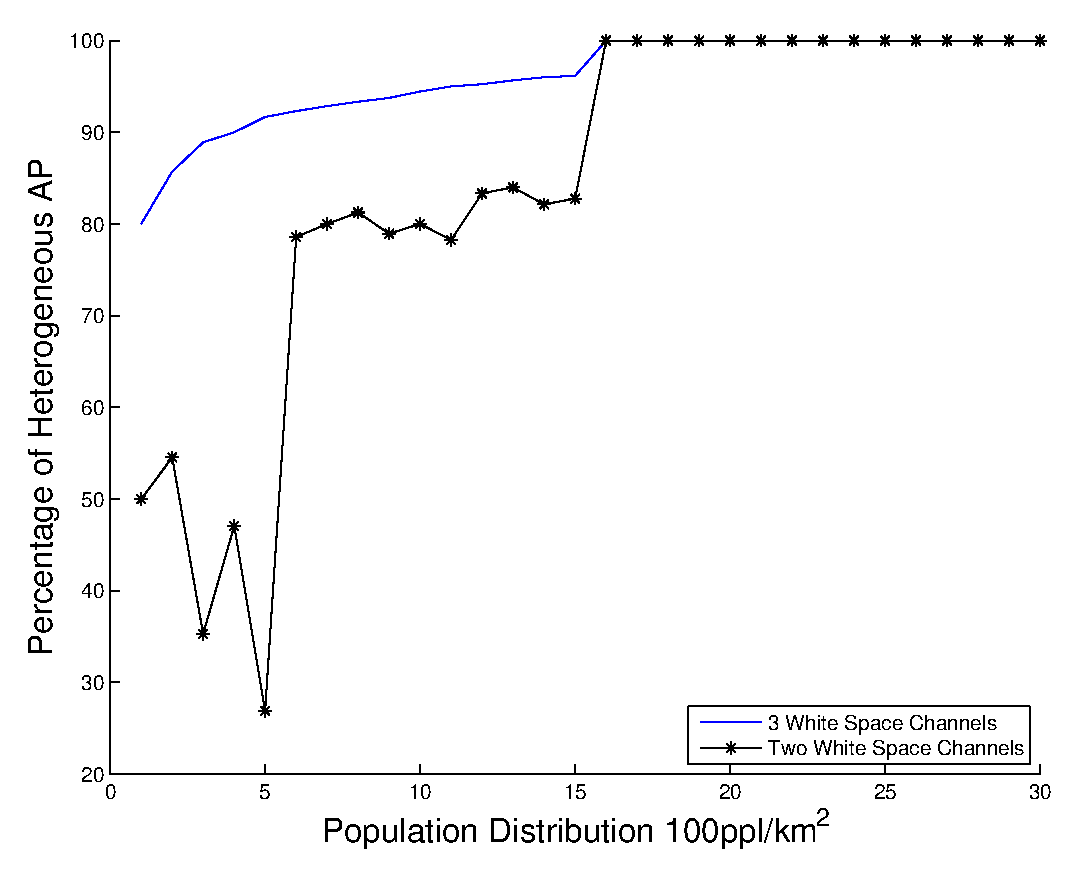
\includegraphics[width=74mm]{figures/percentage}
\vspace{-0.1in}
\caption{Percentage of Heterogeneous Access Points}                                                                 
\label{fig:heappercentage}
\vspace{-0.1in}
\end{figure}

% sum
As shown in the numerical simulation, the heterogeneous access point could balance
the spatial reuse and large service area to adapt multiple traffic demand scenarios.
The combination of white space bands and WiFi bands could reduce the cost for
network deployment significantly.






